%% In a thesis, every section/chapter starts a new page, hence the \clearpage
\clearpage

\section{Background}
\label{sec:background}

This section gives an overview of the areas that are required to evaluate the security of an OAuth system.
Since the OAuth specification deals with transmitting sensitive data over the internet, the first section describes how network communication can be secured, with details on public key encryption and Transport Layer Security.
The second section describes the structure of web applications, considering the different implementation options that are available today as well as their security considerations.
To be able to evaluate different methods for storing OAuth user identifiers, the third section details the different options that are available for storing data in web clients.
The fourth section describes different methods that can be used to authenticate HTTP communication.
The fifth section describes cross-site request forgery attacks, which is a common attack type that is especially relevant in the context of OAuth.


\subsection{Securing network traffic}
The complex and distributed nature of the internet causes it to be inherently insecure. A network request may travel through switches located in a number of countries and operated by various actors, and the route might even change between requests as the network topology and load changes. As such, we have to assume that some link along the chain is listening to the traffic we send. In the context of web traffic, this lack of trust causes issues, as users want to be able to send potentially sensitive information with the knowledge that no external actor will be able to read or modify the data.

\subsubsection{Public key encryption}
To mitigate the risk of malicious parties being able to listen in on network communication, public-key encryption can be used.
Public key cryptography relies on a public-private key pair, where the public key is used to encrypt data and the private key is used to decrypt data.
A network actor can generate the key pair and send the public key to the other endpoint.
Since the public key can only be used to encrypt data, an attacker will not gain any valuable information if they are able to intercept the public key.
With the public key, the other endpoint can encrypt the data before sending it over a network.
Since the data can only be decrypted by the corresponding private key, a network attacker which successfully intercepts the communication is unable to read the original data \citep{hellman_overview_1978}.

Diffie-Hellman key exchange is one method to exchange keys for public key cryptography \citep{diffie_new_1976}  \citep{gillmor_negotiated_2016}.
\begin{enumerate}
    \item The Diffie-Hellman key exchange begins by two parties, Alice and Bob, agreeing on two publicly shared values, $p$, and $g$, where $p$ is a prime and $g$ is a primitive root modulo $p$.
    \item Alice chooses a secret integer $a$ and sends $A = g^a \mod p$ to Bob.
    \item Bob chooses a secret value $b$ and sends $B = g^b \mod p$ to Alice.
    \item Alice computes $s = B^a \mod p$
    \item Bob computes $s = A^b \mod p$
\end{enumerate}

Alice and Bob now share the secret $s$, since \[A^b \mod p = g^{ab} \mod p = g^{ba} \mod p = B^a \mod p\]
The secret share is considered secure, as finding $a$ and $b$ given $g^{ab} \mod p = g^{ba} \mod p$ takes a long time to compute with our current algorithms.

If Diffie-Hellman key exchange is used, an attacker can store large amounts of network traffic, with the hope of the secret key leaking in the future, thus allowing the attacker to decrypt all previous communication.
Additionally, in traditional public-key cryptography, the keys between two parties can stay constant for long amounts of time, allowing an attacker to decrypt all previous traffic at once if the secret is leaked in the future.
To protect against such attacks, short lived keys, commonly referred to as ephemeral keys, can be used, such as in the SAKE protocol \citep{jarecki_symmetric-key_2020}.
The SAKE protocol solves the issue of a future key leak being able to decrypt previous communication by continuously updating the secret key, making it impossible to derive an older secret key from a newer one.
Ensuring that an encryption scheme is resistant to keys being leaked at a later point is known as perfect forward secrecy.

\subsubsection{Transport Layer Security}
Today, the Transport Layer Security (TLS) protocol is used to prevent eavesdropping, tampering and forging messages in client-server communication. The latest version of the specification is TLS 1.3, which among other things removes insecure ciphers, allows for fewer round trips in the handshake and forces clients and servers to use ephemeral key exchange methods, ensuring perfect forward secrecy \citep{dowling_cryptographic_2015}. 

TLS provides a secure channel which provides authentication, confidentiality and integrity, even if an attacker has complete control of the network. The server is always authenticated, while the client can be optionally authenticated. The confidentiality of the transmitted data is ensured by encryption, only allowing the server and client to decrypt the contents. TLS 1.3 additionally ensures forward secrecy, effectively preventing attacks that store large amounts of encrypted data with the hope of decrypting it at a later point when keys are compromised. The lengths of the data and the identities of the client and server are however not hidden. Integrity is ensured by detecting any external modifications to the sent data.

The full TLS 1.3 handshake, described in figure \ref{tls}, functions as follows \citep{rescorla_transport_2018}:

\begin{figure}[b]
	\centering
	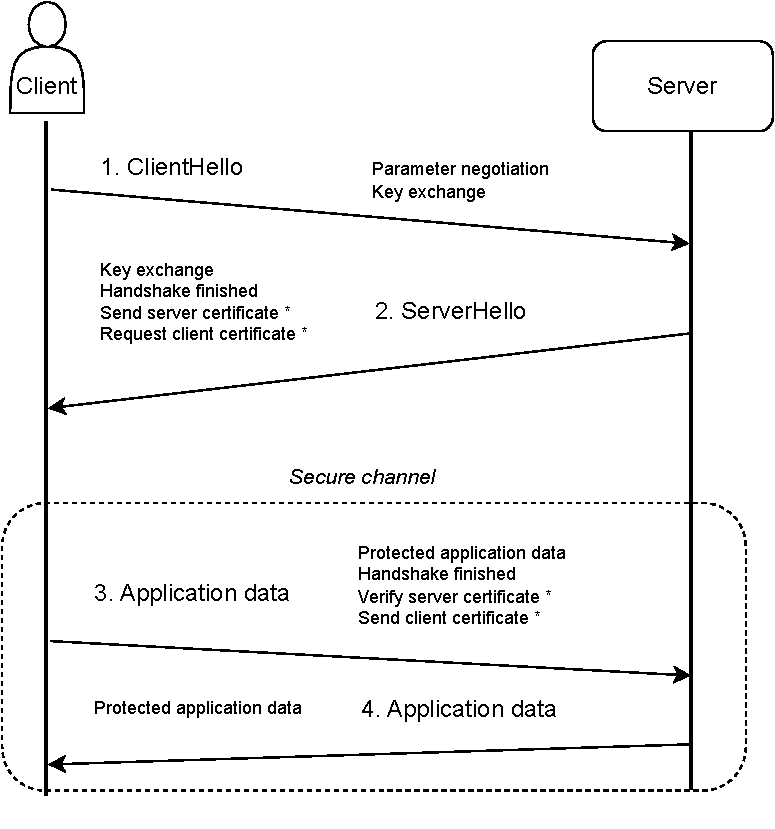
\includegraphics[height=120mm]{assets/tls_1.3_handshake.drawio.pdf}
	\caption{Full TLS 1.3 handshake. Optional content marked with *.}
	\label{tls}
\end{figure}

\begin{enumerate}
    \item The \textit{ClientHello} message is used for negotiating parameters and exchanging keys. The configurable parameters are TLS versions, groups, cipher suites and certificate authorities. The key exchange is initiated by sending the client's Diffie-Hellman key share. The client can request a server certificate, further ensuring that no impersonation attack can take place.
    \item \textit{ServerHello}: The server selects a cipher and TLS version based on the lists sent by the client and confirms that the handshake is finished. The server can suggest new parameters if it does not support any of the parameters sent by the client. The server also sends its own Diffie-Hellman key share and a server certificate, if one was requested. If client authentication is used, the server will request a client certificate. If a pre-shared key is used, the server can send application data in this message, allowing for data transfer without any additional round trips.
    \item A secure channel is established, allowing the client to send application data encrypted with the previously shared key. The client confirms that the handshake has been completed and sends a certificate if one was requested.
    \item The server can now use the secure channel to send encrypted application data.
\end{enumerate}

\clearpage
\subsection{Structure of web applications}
\label{sec:background-structure}

Web pages can be characterized by clients fetching web pages from servers and displaying the pages in web browsers. The basic building blocks for a web page are HyperText Markup Language (HTML) elements, which describe the structure and content of the page. The layout and style of web pages can be modified by using Cascading Style Sheets (CSS). The addition of JavaScript makes it possible for the browser to execute arbitrary code, greatly improving the options for interactive pages. 
Since its inception in the 80's, the web has evolved and matured. From static, read-only pages utilizing HTML to pages allowing users to write and participate in the web during the turn of the millennium, made possible in part by the adoption of JavaScript. The evolution continued to allow users to execute programs that we commonly refer to as web applications today \citep{jacksi_development_2019}. 


\subsubsection{Static web pages}
A traditional, static web page is stored in its entirety on the server and is served to users on request. 
Such pages typically require only HTML and CSS to function.
As the client side barely includes any logic, the focus is on the server, which stores and serves data and handles all business logic.
Navigation and interaction with the page is done using clickable links that direct the user to other pages.
Figure \ref{static} describes a user visiting a web page \textit{example.com}, clicking a link to visit \textit{example.com/apply} and finally submitting a form to \textit{example.com/apply}.
Keeping the content strictly separated in pages and serving the complete page as-is to clients provides a number of benefits \citep{camden_why_nodate}:

\begin{itemize}
    \item The amount of data transferred when visiting a site is low, as only the content that is immediately shown to the user has to be sent. This speeds up load times for the end user, reduces data usage and typically leads to a lower delay before content is visible in the browser.
    \item Static websites are typically easier to traverse programmatically than dynamic sites. This makes it easier for web crawlers to index the site, such as those used by search engines, making search engine optimization (SEO) trivial. Additionally, static sites are typically more accessible as they can be parsed more easily by screen readers and similar software \citep{okoye_accessibility_2014}.
    \item As the use of JavaScript allows websites to execute near arbitrary code in browsers, users can choose to disable JavaScript altogether. This will cause most dynamic sites to stop working, while static websites can function without using JavaScript. This removes the option for potential attackers to execute harmful code on the user's machine and often limits the tracking capabilities of websites. 
\end{itemize}

There are, however, reasons why strictly static sites are rare today, compared to the early days of the web when they were the standard \citep{nath_web_2014}:

\begin{itemize}
    \item Static websites are slow and clunky to use, as any interaction with the site requires the client to fetch a new page, or reload the current page from the server.
    \item Static websites only support client-initiated requests, making it impossible for the server to implement event-driven patterns, such as sending notifications to the client.
    \item Continually updating pages is not possible, as doing so would require server-initiated communication. The problem could be solved by the client periodically requesting the latest data, but this is not possible in strictly static sites as it requires JavaScript to implement.
\end{itemize}

\begin{figure}[b]
	\centering
	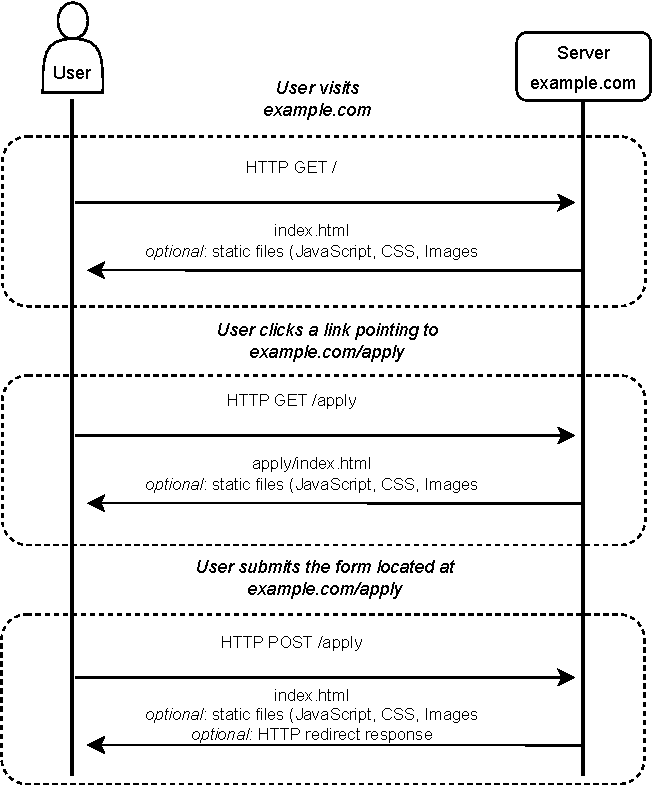
\includegraphics[height=120mm]{assets/http_request.drawio.pdf}
	\caption{Network traffic for a user interacting with a static web site.}
	\label{static}
\end{figure}

\subsubsection{Rich internet applications}

To allow for client-side scripting and alleviate some of the issues with strictly static sites, JavaScript was introduced in the mid 90's. While this allowed developers to create dynamic user interfaces, web apps as we know them today did not become popular until the introduction of third-party tools, such as Adobe Flash and Java in web apps. These technologies allowed for the development of rich internet applications (RIAs) that delegated some logic and data storage to the client, while using separate HTML pages for different pages \citep{fraternali_rich_2010}.
While these tools allowed for the creation of interactive web apps, end users had to install the tools separately if they wanted to utilize them. In addition to being a hassle for end users, these plugins introduced additional security vulnerabilities. At the time of writing, 1084 common vulnerabilities and exposures (CVEs) have been reported for Adobe Flash \citep{noauthor_adobe_nodate}.

Some way to create interactive web apps using only HTML, CSS and JavaScript was needed. The adoption of Asynchronous JavaScript and XML (Ajax) around 2005 saw web development move towards JavaScript-based applications that are common today. 
The asynchronous nature of Ajax allowed for completing network requests in the background without blocking user input and updating relevant parts of the interface when the request completed. 
JavaScript-based abstractions built on top of Ajax made development easier, such as jQuery \citep{openjsforg_jquery_nodate}, released in 2006, and the fetch() function \citep{noauthor_fetch_2023}, released in 2015. 

\subsubsection{Single-page applications}

Logic can further be delegated to the client, allowing for single-page applications (SPAs), that contain all the web pages for an application in one HTML page
\citep{fink_introducing_2014}. 
While the name might imply that SPAs only have one page, they can have any number of pages visible from the end users point of view, with the term \textit{single page} referring to the number of HTML pages.
In contrast to static web applications and RIAs, SPAs use client side logic instead of full HTTP requests to handle navigation and user input.
This often leads to improved responsiveness for users and makes dealing with client-side data and state easier, at the cost of a longer initial load time due to the larger size of the page.
The backend typically consists of an application programming interface (API), which is designed for machine communication with responses that might not be easily human-readable.
The backend and frontend often utilize JavaScript Object Notation (JSON) data to communicate.

Figure \ref{spa} shows the network traffic between a user and a web server for a simple SPA.
When comparing the traffic with the static page traffic in figure 2, the static page always returns a complete HTML page and redirects the user accordingly, while the SPA only fetches one HTML page on the initial page load.
The requests for the user navigating to \textit{/apply} and the user submitting a form can be identical for both the static page and the SPA.
The response from the backend is however different, with the static application returning a complete page and the SPA returning data in any suitable format, typically JSON.

\begin{figure}[b]
	\centering
	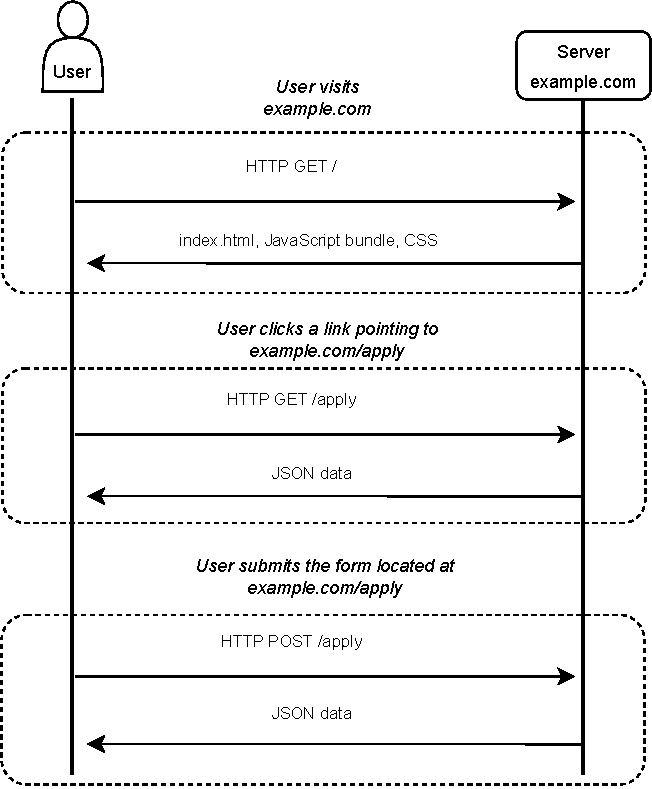
\includegraphics[height=120mm]{assets/spa_http_request.drawio.pdf}
	\caption{Network traffic for a user interacting with a Single Page Application.}
	\label{spa}
\end{figure}

While the network traffic of the SPA and static web page might seem very similar at first, there are many practical differences \citep{fink_introducing_2014}.
As SPAs implement navigation in the client, user navigation could be achieved without any network traffic, completely relying on the content of the first page load.
In practice some network traffic is often useful when navigating a SPA. 
Dynamic information can be fetched on navigation, periodically by the client or on-demand by the server, as data fetched on initial page load could easily become stale.
Pre-rendered HTML and static content such as images can also be fetched on navigation, lowering the size of the initial HTML page.
With SPAs, developers are given greater freedom in implementation, having the option to develop web applications very similarly to native applications, while not requiring end users to install anything on their machines.
While moving much of the logic to the client can make applications more responsive, moving logic from an opaque server to a transparent client application requires developers to pay attention to which parts they could move to the client.
In general, developers should assume that all data and application logic that is located in the client can be freely accessed and modified by potential attackers.


\subsection{Client-side storage}
\label{sec:background-storage}

In web applications that execute code on the client, storing data in the client browser is often required.
The use of JavaScript allows developers to store data in variables, making it possible to keep track of application state and to create more complex programs.
It is often useful to persist data over different sessions, and as JavaScript variables are cleared when refreshing the page, other methods for storing data are needed.
A common use case for persistent storage methods is keeping track of users by storing a session token in the client browser, allowing authenticated users to navigate a web page without having to authenticate every time they visit a new page.

\subsubsection{Cookies}
\label{sec:background-storage-cookies}
Cookies have long been used to allow servers to store state at HTTP user agents, such as web browsers, over the HTTP protocol, which itself is mostly stateless.
Cookies function by passing data in HTTP headers.
By using the Set-Cookie field, servers can pass name/value pairs and related metadata to user agents.
In later requests, the user agent can set a previously stored value in the Cookie field, allowing the server to identify the client or to keep track of user preferences.
Cookies are not always suitable for keeping track of user state or identifiers.
Using cookies, a server cannot differentiate between different sessions for one user.
As an example, if a user had two separate windows open at the same time and was trying to purchase two different items, the session would leak between the two windows \citep{noauthor_html_nodate}.
Cookies are also limited by their max size, which is 4096 bytes.

When setting cookies, the server can define the scope of the cookie, which can include the domain and path of the cookie, as well as if it should be allowed to be used in HTTP requests that do not use TLS
\citep{barth_rfc6265_2011}.
The use of scope for cookies is essential if it contains confidential information such as session identifiers.
If a domain is not defined for the cookie, the value could be read by any visited website, significantly increasing the chance for session hijacking.
Similarly, if the cookie is allowed to be used without TLS, any network attacker would be able to read the transmitted data.
To limit many vulnerabilities, such as cross-site scripting (XSS) attacks, the \textit{HttpOnly} flag can be set for cookies that are used as session identifiers.
The flag blocks access to the cookie from JavaScript executed in the client, only allowing it to be sent as part of a request in the Cookie header.

To further protect against cross-site attacks, the \textit{SameSite} attribute can be used \citep{khodayari_state_2022}.
Three different \textit{SameSite}  policies exist: None, Lax and Strict.
A cookie with the None policy is attached to all outgoing requests, which includes cross-site requests.
Cookies with the Lax policy are attached to same-site requests as well as cross-site requests with safe HTTP methods, which includes using the HTTP GET method and the request resulting from a top-level navigation by the user, such as clicking on a link.
Cookies with the Strict policy are only included on requests that originated from the same origin.
As such, if a user clicks a link to a site on a page with some other origin, the cookie will not be included.

\subsubsection{Web storage API}
The web storage API was created to deal with some of the issues of cookies.
The API includes two mechanisms for storing data, session storage and local storage \citep{noauthor_html_nodate}.
Both storage methods allow persisting data for longer periods of time, while also separating the storage by domain.
As data is unencrypted at rest, the web storage API is inherently insecure.
Additionally, web storage is vulnerable to a number of attacks, such as XSS attacks, requiring developers to implement additional security features and considering what kind of data to store.
Due to these security concerns, web storage should not be used to store any sensitive data.
Session storage persists data for the lifetime of the session, keeping the data through page navigations and refreshes until the browser or tab is closed \citep{noauthor_web_2023}.
Local storage persists data over multiple sessions, having to be explicitly cleared by using JavaScript or by clearing all browser storage.


%\begin{itemize}
%    \item IndexedDB?
%    \item cache?
%    \item Storing in files on the client?
%    \item service worker?
%\end{itemize}

\subsection{Authenticating HTTP requests}
As internet-facing applications can be accessed by anyone, it is often necessary to authenticate entities trying to communicate with the application.
Authentication can be used for limiting access to only certain users or to display user-specific information.
As the authenticated entities can vary from human users to devices or other servers, different ways of authentication can be appropriate for different systems.
In a traditional web application with a client, a backend and a database, the authenticated parties are typically the client when communicating with the backend and the backend when communicating with the database.

The need for authenticating HTTP requests has existed since the early days of the internet, with the basic HTTP authentication scheme being an early method \citep{reschke_basic_2015}. 
Basic authentication functions by sending an authorization header with a base64-encoded string containing a username and password, which the server can use to identify the user, by comparing the string with a stored value, which should be encrypted at rest.
Notably, the scheme does not provide any confidentiality for credentials, as the credentials are not encrypted or hashed in any way, allowing for the base64 value to be easily decoded.
While the encryption of headers in TLS prevents outside attackers in the network from reading the credentials, this lack of confidentiality allows the receiving server to access the plain text credentials.
This allows hostile or compromised servers to capture credentials which can be used on other sites in the case of credential reuse.
A 2014 study by Das et al. found that 43\% of users directly reuse passwords on different sites \citep{das_tangled_2014}.
With these issues and the prevalence of password reuse in mind, the basic HTTP scheme can no longer be considered appropriate for many web applications.

Human-readable passwords are not always required, and in many cases API keys can be appropriate for authenticating clients \citep{farrell_api_2009}.
API keys differ from basic authentication by only identifying users by a single secret string that is shared between the client and server, instead of a string and a username.
As developers can define the authentication string freely, it could in theory be constructed similarly to the string used in basic authentication.
In practice, the API key is often a completely random string, with the server keeping a track of who the string belongs to if required.
The API key can also be a hashed string similar to the one used in basic authentication, allowing the storage of a user identifier and password without the risk of leaking either the password or the user identifier.
Similarly to basic authentication, API keys are sent in a request header, often using the X-API-KEY header.
The API key could also be sent as a query parameter or in the request body itself depending on the implementation.
API keys are especially useful if the server does not need to differentiate between clients, if there are a small number of clients or if the client is not a user-facing web client, such as a backend server communicating with an external API.
While API keys mitigate some of the risks associated with sending unencrypted passwords over the internet, they suffer from many of the same flaws as basic authentication.
Similarly to basic authentication, the API key is the same for each request and as such it only has to be leaked once for attackers to gain unapproved access.
While systematically rotating API keys can lower the risk of the API keys leaking, they are not optimal for all use cases today.

Both of the described authentication schemes share the weaknesses of requiring servers to store the user identifiers and reusing the same identifier for an unspecified amount of time.
Servers also have to implement the authentication logic separately, leaving room for poor implementations and suboptimal credential storage.
Token-based authentication has become a popular way to outsource the authentication logic to a trusted third party.
Token-based authentication functions by redirecting the user to an identity provider (IdP) which authenticates the user and grants a token identifying the user \citep{hardt_oauth_2012}.
A token can be a random string with sufficient length to make it unlikely for a third party to be able to guess it.
A token can contain some information about the user, but it can also be completely opaque.
The client can store this authentication token and send it with any future request, typically as a cookie (described in section \ref{sec:background-storage-cookies}), allowing servers to verify the user by querying the IdP with the user token.
Compared to the static API key, authentication tokens are typically only valid for a short amount of time, mitigating the risk of credential hijacking.
To remove the need for users to log in continuously, access tokens can often be refreshed silently in the background by the client application.




\subsection{Cross-site request forgery}
Cross-site request forgery (CSRF) is an attack where an attacker causes a victim's browser to perform an unwanted operation on a trusted website.
CSRF attacks rely on the fact that stored user sessions belonging to a specific domain tend to be included automatically in all HTTP requests to the domain.
As such, if the victim is tricked to click a link to the target site with some malicious payload, such as a form submission to update a password, the victim's browser will automatically include the victim's session in the request, allowing the attacker to perform operations as the victim.
A typical CSRF attack has the goal of gaining access to resources belonging to the victim \citep{lin_threat_2009}.
This can give attackers access to private resources belonging to the victim or allow attackers to impersonate the victim.
By forging a request that signs the victim in as the attacker to a legitimate site, a victim can be tricked to perform operations as the attacker in \citep{barth_robust_2008}.
These login CSRF attacks are more difficult to defend against than traditional CSRF attacks but can be equally damaging.
An attacker could for example trick the victim to store a payment method in the attackers account.

CSRF attacks can be performed using a number of methods that all rely on somehow causing the victim's browser to visit a link provided by the attacker.
In an ideal case for the attacker, the vulnerable route is a HTTP form that allows the attacker to perform an operation as the victim, such as transferring money or changing account passwords.
On a website with user-generated content, such as a forum, attackers could embed malicious links in images.
For malicious images to be executed on page load the site will need to have a vulnerable route where a HTTP GET request executes an operation with side-effects.
According to the HTTP specification, GET requests should be free of side effects, but it is up to developers to correctly implement the specification.
If a victim visits a malicious site controlled by the attacker, the malicious site can instruct the user's browser to execute any HTTP request to the vulnerable site.
Compared to the malicious embedded images, the target site does not need to have any wrongly configured routes that execute GET requests with side-effects, as the attacker can freely choose the type of HTTP request.

As the potential for CSRF attacks have been known for many years, a number of well-known defenses exist.
Bart et al. (2008) suggest protecting against CSRF attacks by using secret validation tokens \citep{barth_robust_2008}.
A secret validation token is a random value that is included by applications in each HTTP request to ensure that requests have been sent from an authorized source.
The token should be hard to guess for attackers that do not already have access to the victim's account.
As the token will have to be stored in the client, end users will be able to access it with ease in many cases.
As such, the token should never be shared between user or sessions, and should ideally be treated as a single-use nonce to make replay attacks less likely.


